%-------------------------------------------------------------------------------
\section{The model}\label{sec:model}
%-------------------------------------------------------------------------------
In this section, the atmospheric model used for \mf\ is described in
more detail. First, the building and properties of the atmospheric profiles
required for the calculation of emission and absorption spectra are discussed
(Section~\ref{sec:profiles}). Then, we explain the properties of the
radiative transfer code used (Section~\ref{sec:radcodes}). The contribution of
the different molecules to the resulting atmospheric spectra is discussed in
Section~\ref{sec:spectra}. Moreover, we provide some information on the
modelling of the telescope emission (Section~\ref{sec:greybody}). Finally, we
describe how the resulting model is adapted to the input science spectrum
(Section~\ref{sec:adaption}).

%-------------------------------------------------------------------------------
\subsection{Atmospheric profiles and meteorological data}\label{sec:profiles}
%-------------------------------------------------------------------------------
Information concerning the composition of the atmosphere is available at
various levels. To the end of creating a uniform profile with the variables
temperature, pressure, and density of various molecular species as a function
of geoelevation, three sources of input are merged: standard profile
(produced for \ac{MIPAS} onboard the ENVISAT satellite), \ac{GDAS} profile, and
\ac{EMM} data.

The largest amount of molecular density information is contained in the
atmospheric standard profiles. However, they are only available for specific
geographical latitudes and do not contain any time information whatsoever
(see Section~\ref{sec:mipas}). To compensate the lack of time information, one
can rely on the EMM (see Section~\ref{sec:emm}). It provides the most frequent
updates and is specific to the selected observing site. Unfortunately, it
cannot provide molecular species information apart from water vapour (relative
humidity measurements) and is restricted to a local on-site measurement, \ie\
a single geoelevation data point only. To bridge the gap between these two data
sources, \ac{GDAS} provides a global grid of profile measurements (with
approximate grid spacing of 110\,km) to an altitude of $\sim$\,26\,km with
updates every three hours. \ac{GDAS} does not contain molecular species apart
from H$_2$O, though (see Section~\ref{sec:gdas}).

These three data sources and the required processing for use with \mf\ are
described in detail below (see also Noll et al. \cite{NOL12}).

%-------------------------------------------------------------------------------
\subsubsection{MIPAS profiles}\label{sec:mipas}
%-------------------------------------------------------------------------------
The atmospheric standard profiles provide the basis for the model atmosphere
used in \mf\ (see parameter {\sc ref\_atm} in Section~\ref{sec:params})
including information on pressure, temperature, and molecular abundance as
function of height (121 levels in the range 0-120\,km). Up to now, the
\ac{RFM} homepage \cite{RFM} provides standard profiles for mid-latitude
(Lat~$ = 45^\circ$, both, day and night), polar winter/summer (Lat~$ = 75^\circ$)
and equatorial day-time conditions in such a configuration (J. Remedios 2001).
So far, the following molecules are included in this standard profile: N$_2$,
O$_2$, CO$_2$, O$_3$, H$_2$O, CH$_4$, N$_2$O, HNO$_3$, CO, NO$_2$, N$_2$O$_5$,
ClO, HOCl, ClONO$_2$, NO, HNO$_4$, HCN, NH$_3$, F11, F12, F14, F22, CCl$_4$,
COF$_2$, H$_2$O$_2$, C$_2$H$_2$, C$_2$H$_6$, OCS, SO$_2$, and SF (see
Table~\ref{tab:molecs}). Additional molecule profiles for F13 (CClF3), F21
(CHCl$_2$F), F113 (C$_2$Cl$_3$F$_3$), F114 (C$_2$Cl$_2$F$_4$), F115
(C$_2$ClF$_5$), and CH$_3$Cl are available. Apart from these data, less
resolved profiles (a tropical, sub-arctic summer/winter and a US standard
profile) are available with 50 geoelevation layers including the molecules
H$_2$O, CO$_2$, O$_3$, N$_2$O, CO, CH$_4$, and O$_2$ only.

%-------------------------------------------------------------------------------
\paragraph*{Comparison between atmospheric standard profiles}
\label{sec:results_std_profiles}
%-------------------------------------------------------------------------------
In this section, an equatorial day-time \verb|equ.atm| and a mid-latitude
profile \verb|ngt.atm|, corresponding to a latitude Lat~$= 45^\circ$, will
be compared. The location of Paranal (Lat~$= 24.6^\circ$) is between these two
profiles. In Figure~\ref{fig:std_atm_comp} both profiles are shown. Although
the distribution of several molecules (\eg\ N$_2$, O$_2$, CO$_2$) does not
vary, significant differences between the two profiles are visible. To
investigate the impact of the input profile differences on the output spectra,
\ac{LBLRTM} was run with the same input parameters, but with varying standard
profiles.

The resulting spectra are shown in
Figures~\ref{fig:stdcomp_4-28_R}/\ref{fig:stdcomp_4-28_T}. These plots reveal
output radiance spectra differing by at most $\pm 10\%$. The same is true for
the transmission spectra, although somewhat less obvious due to numerical
instabilities. Calculating the broad-band ratios in the main filter ranges
$UBVRI_{\rm c}JHKLMN$ indicates deviations of less than 2\% (see
Table~\ref{tab:std_comp}). Hence, one can conclude that the differences between
the two standard atmospheric profiles are negligible at this stage. Anu Dudhia
\cite[priv.comm.]{anu09}, the author of the \ac{RFM} code, recommends the
equatorial profile \verb|equ.atm| to be used for typical applications at Cerro
Paranal.

%-------------------------------------------------------------------------------
\begin{table}[hb]
\caption[]{Broad-band comparison of the relative ratios between the
{\tt equ.atm} and the {\tt ngt.atm} atmospheric standard profiles.}
\label{tab:std_comp}
\centering
\vspace{5pt}
\begin{tabular}{c @{\qquad} c c c c c}
\hline\hline
\noalign{\smallskip}
Filter & $\lambda_{\rm min}$ & $\lambda_{\rm max}$ & Radiance & Transmission \\
& [\mum] & [\mum] & ratio [\%] & ratio [\%] \\
\noalign{\smallskip}
\hline
\noalign{\smallskip}
$U$ & 0.33 & 0.40 & 0.02 & 0.06 \\
$B$ & 0.39 & 0.50 & 0.00 & 0.02 \\
$V$ & 0.50 & 0.60 & 0.14 & 0.56 \\
$R$ & 0.58 & 0.82 & 0.05 & 0.28 \\
$I_{\rm c}$ & 0.73 & 0.85 & 0.01 & 0.04 \\
$J$ & 1.10 & 1.34 & -0.00 & -0.00 \\
$H$ & 1.50 & 1.80 & -0.00 & -0.01 \\
$K$ & 2.00 & 2.40 & -0.05 & -0.06 \\
$L$ & 3.56 & 4.12 & -0.00 & -0.05 \\
$M$ & 4.52 & 4.96 & -0.69 & 1.37 \\
$N$ & 7.40 & 13.60 & -0.60 & 1.39 \\
\noalign{\smallskip}
\hline
\end{tabular}
\end{table}
%-------------------------------------------------------------------------------
\begin{figure}[ht]
  \begin{center}
    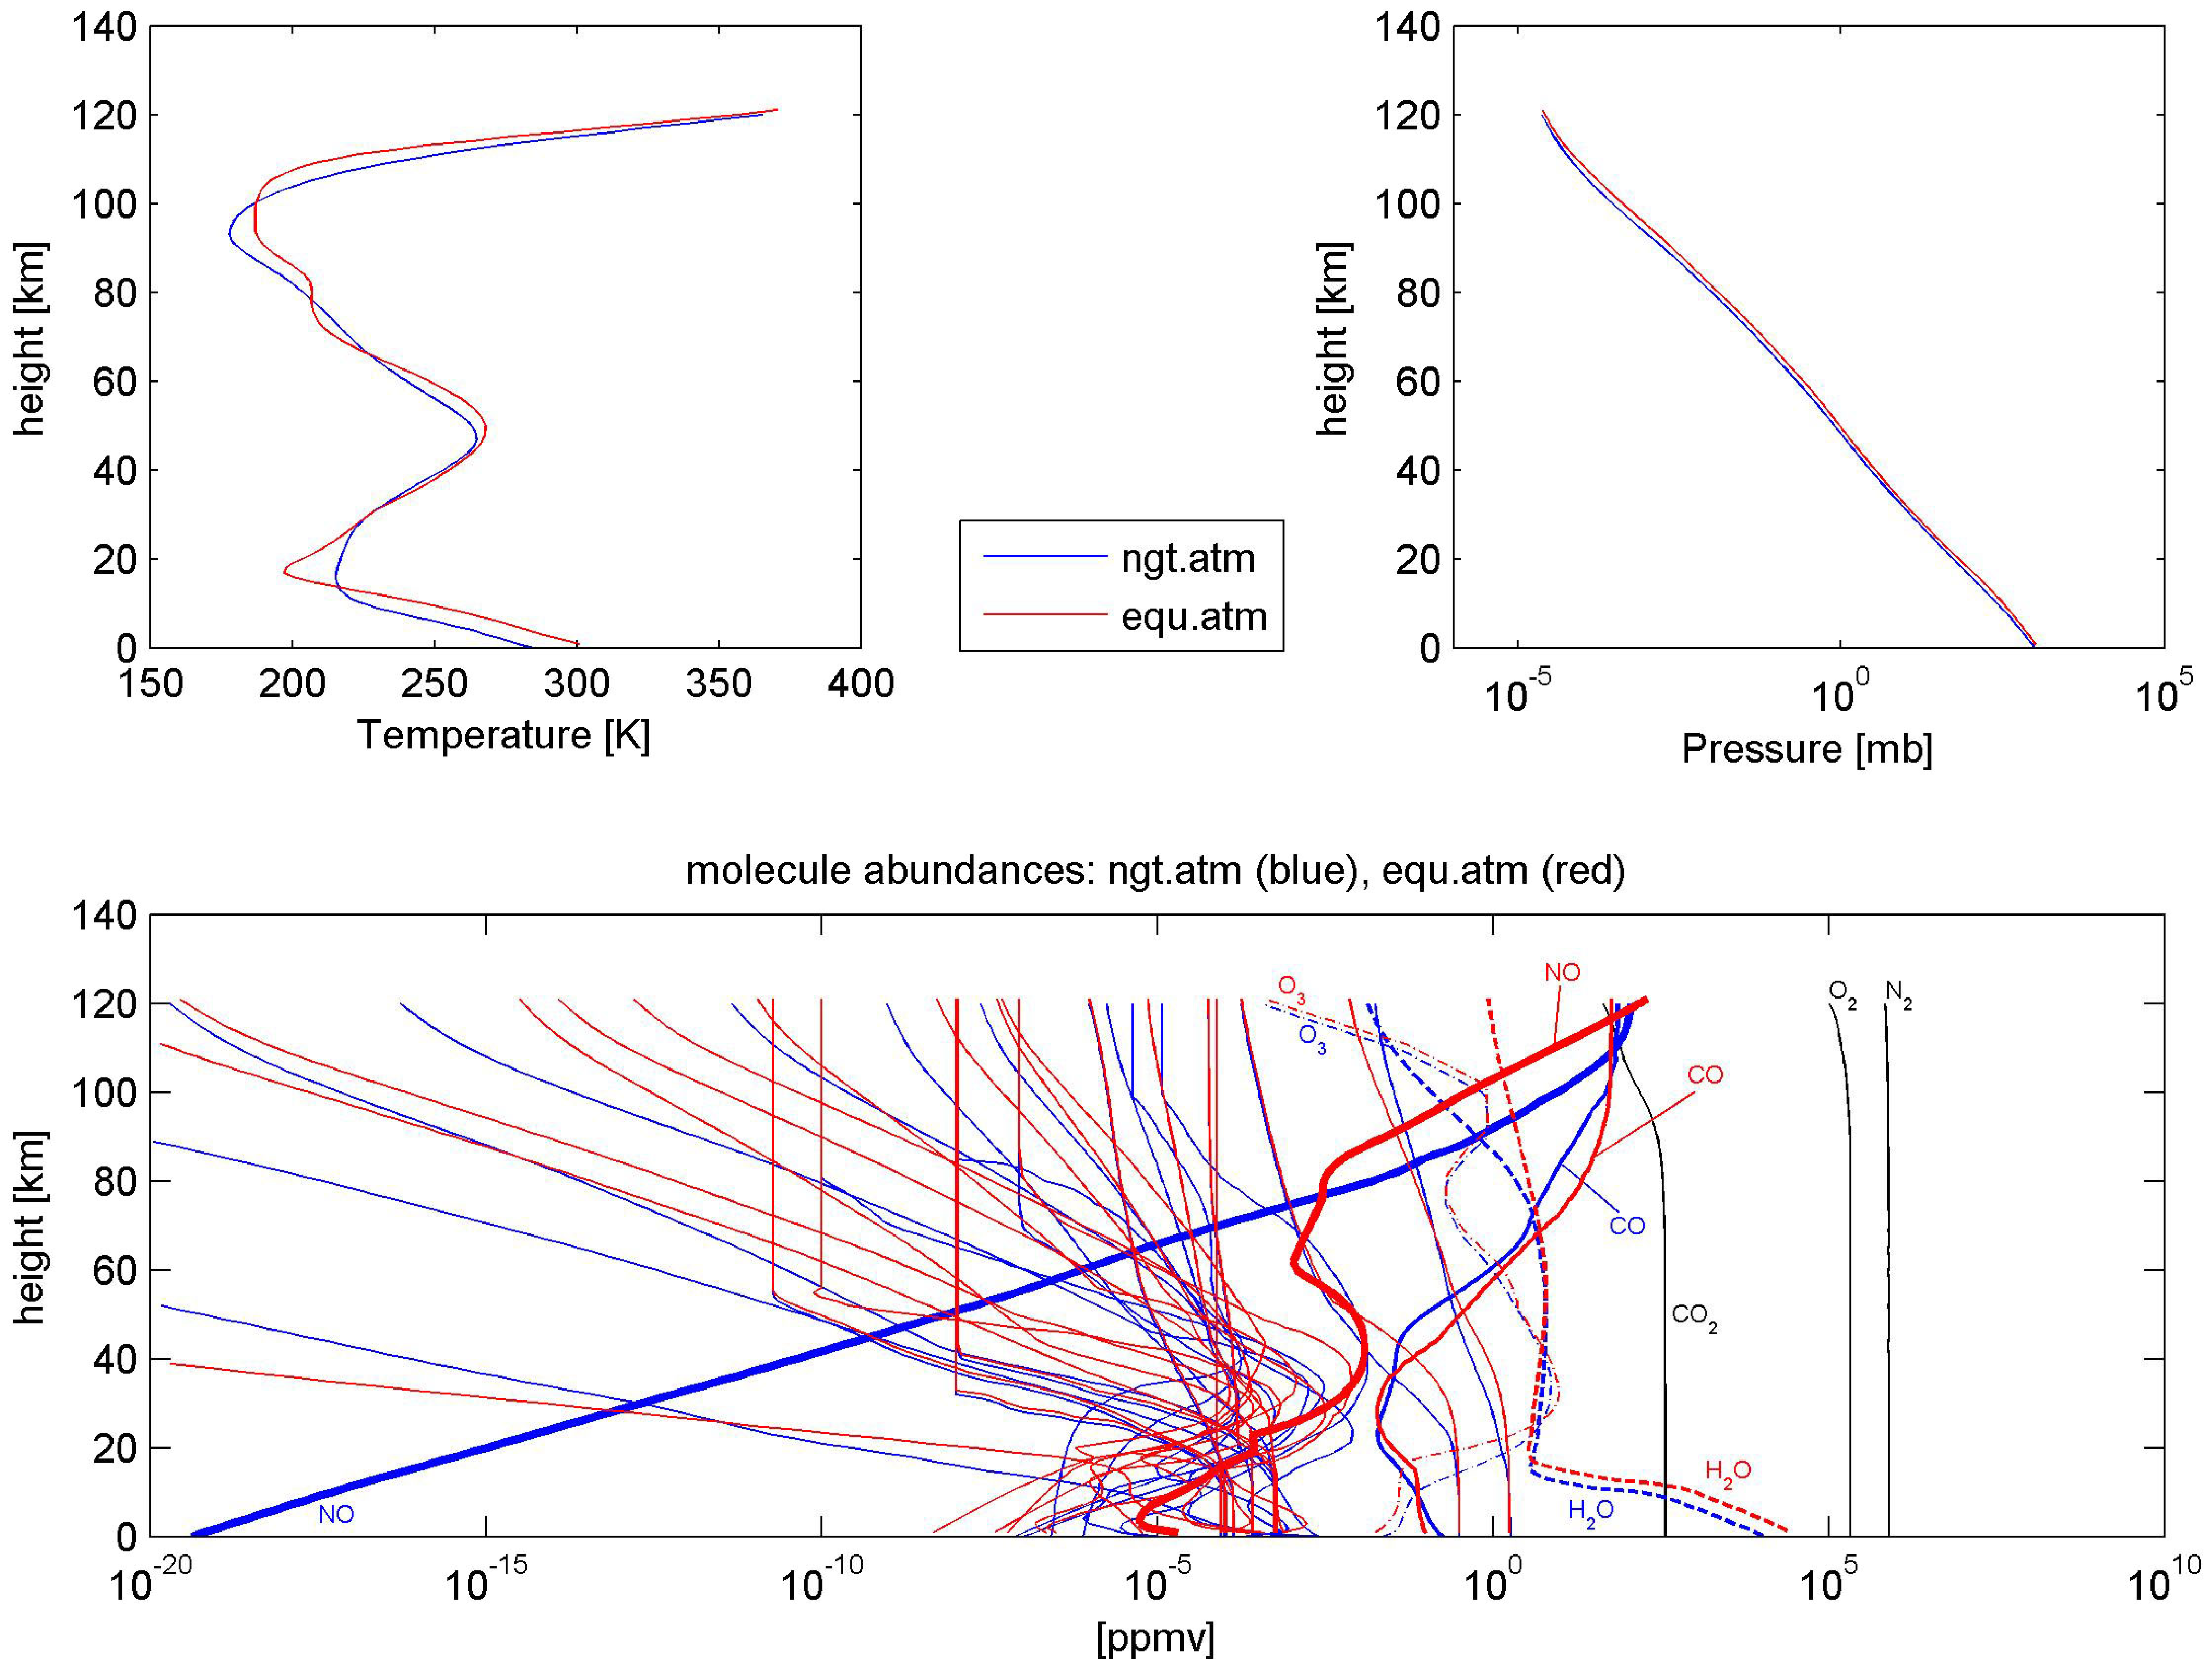
\psfig{file=figures/ngt_equ.eps,width=1.0\textwidth}
    \caption{Comparison of the equatorial (\tt equ.atm\rm) and the mid-latitude
    night time atmospheric profile (\tt ngt.atm\rm). Red lines correspond to
    the equatorial, blue lines to the mid-latitude profile.}
    \label{fig:std_atm_comp}
  \end{center}
\end{figure}
%-------------------------------------------------------------------------------
\begin{figure}[ht]
  \begin{center}
    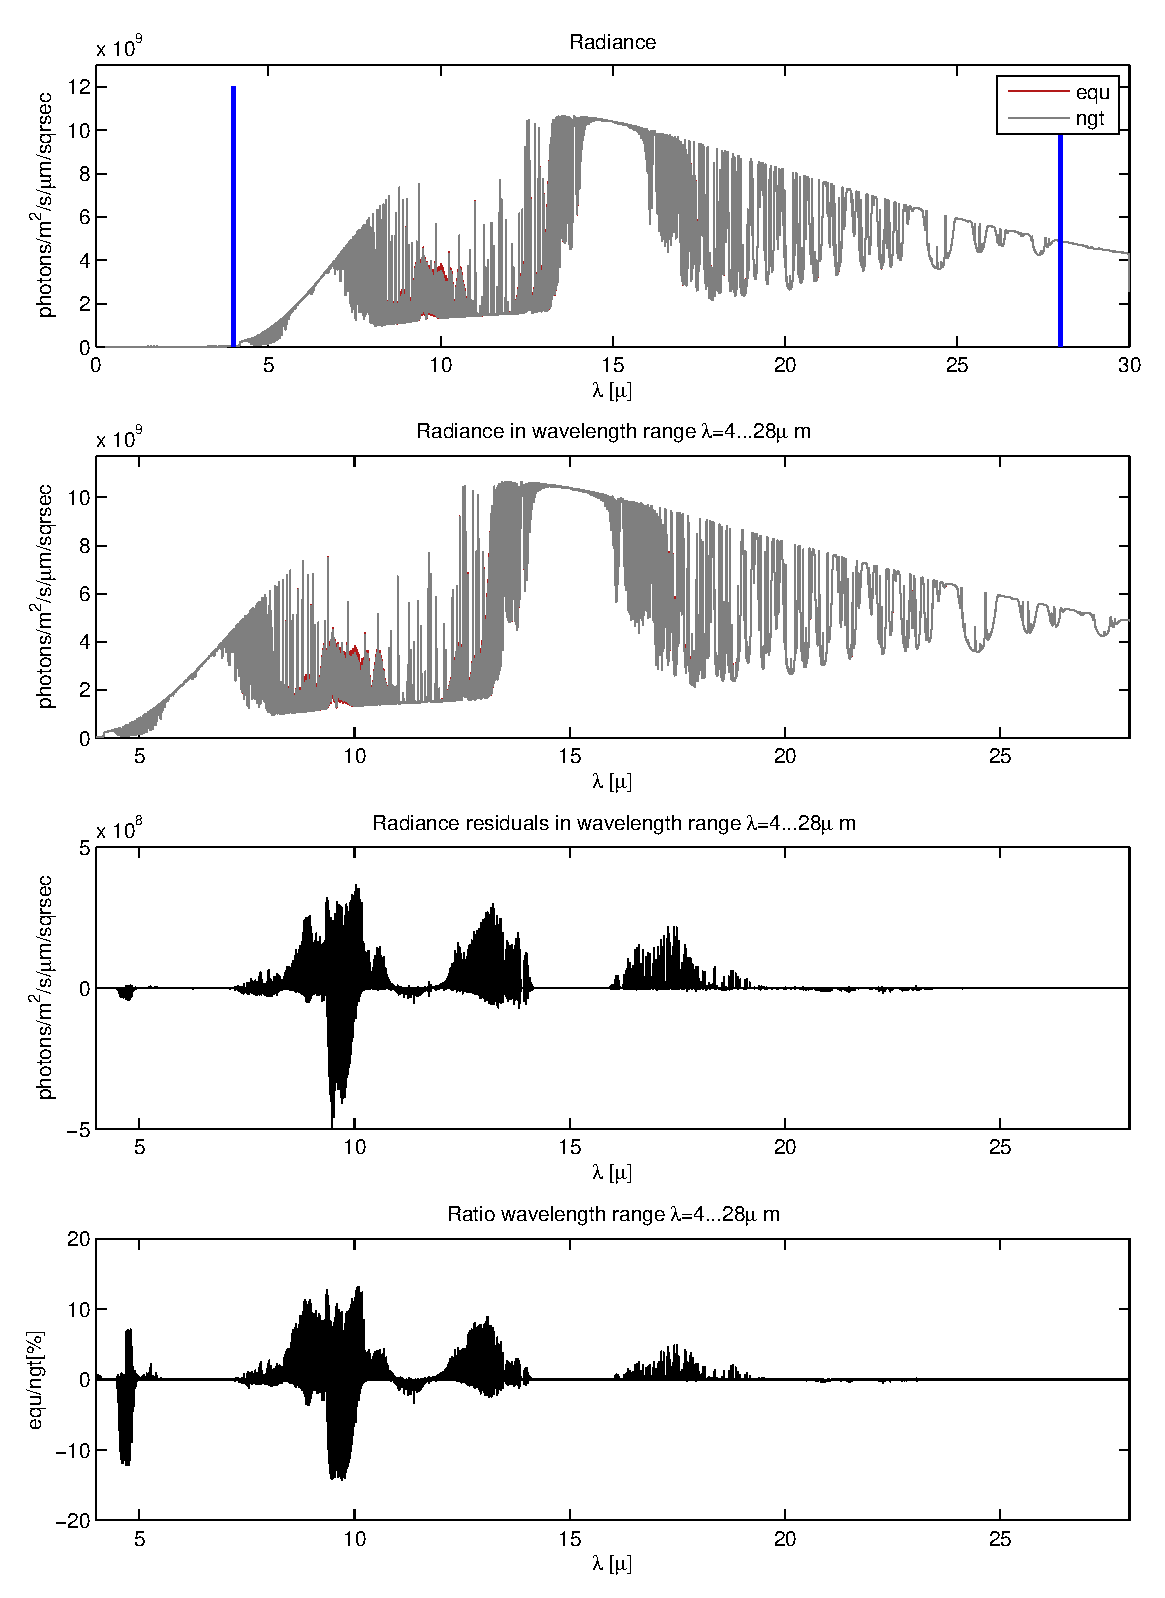
\psfig{file=figures/equ_ngt_4-28mu_rad.eps,width=0.75\textwidth}
    \caption{Direct comparison between the radiance spectra of equatorial day
    time (red line) and mid-latitude night time atmospheric standard profile
    (grey line) over the entire wavelength range $\lambda = 0.3 - 30$\,\mum{}
    (top panel). Blue lines mark the wavelength range
    ($\lambda = 4 - 28$\,\mum) plotted in the three panels below. {\it Second
    panel}: Same as in top panel, but for the limited wavelength range.
    {\it Third and bottom panel}: Residuals equ-ngt and ratio equ/ngt of the
    radiance spectra, respectively.}
    \label{fig:stdcomp_4-28_R}
  \end{center}
\end{figure}
%-------------------------------------------------------------------------------
\begin{figure}[ht]
  \begin{center}
    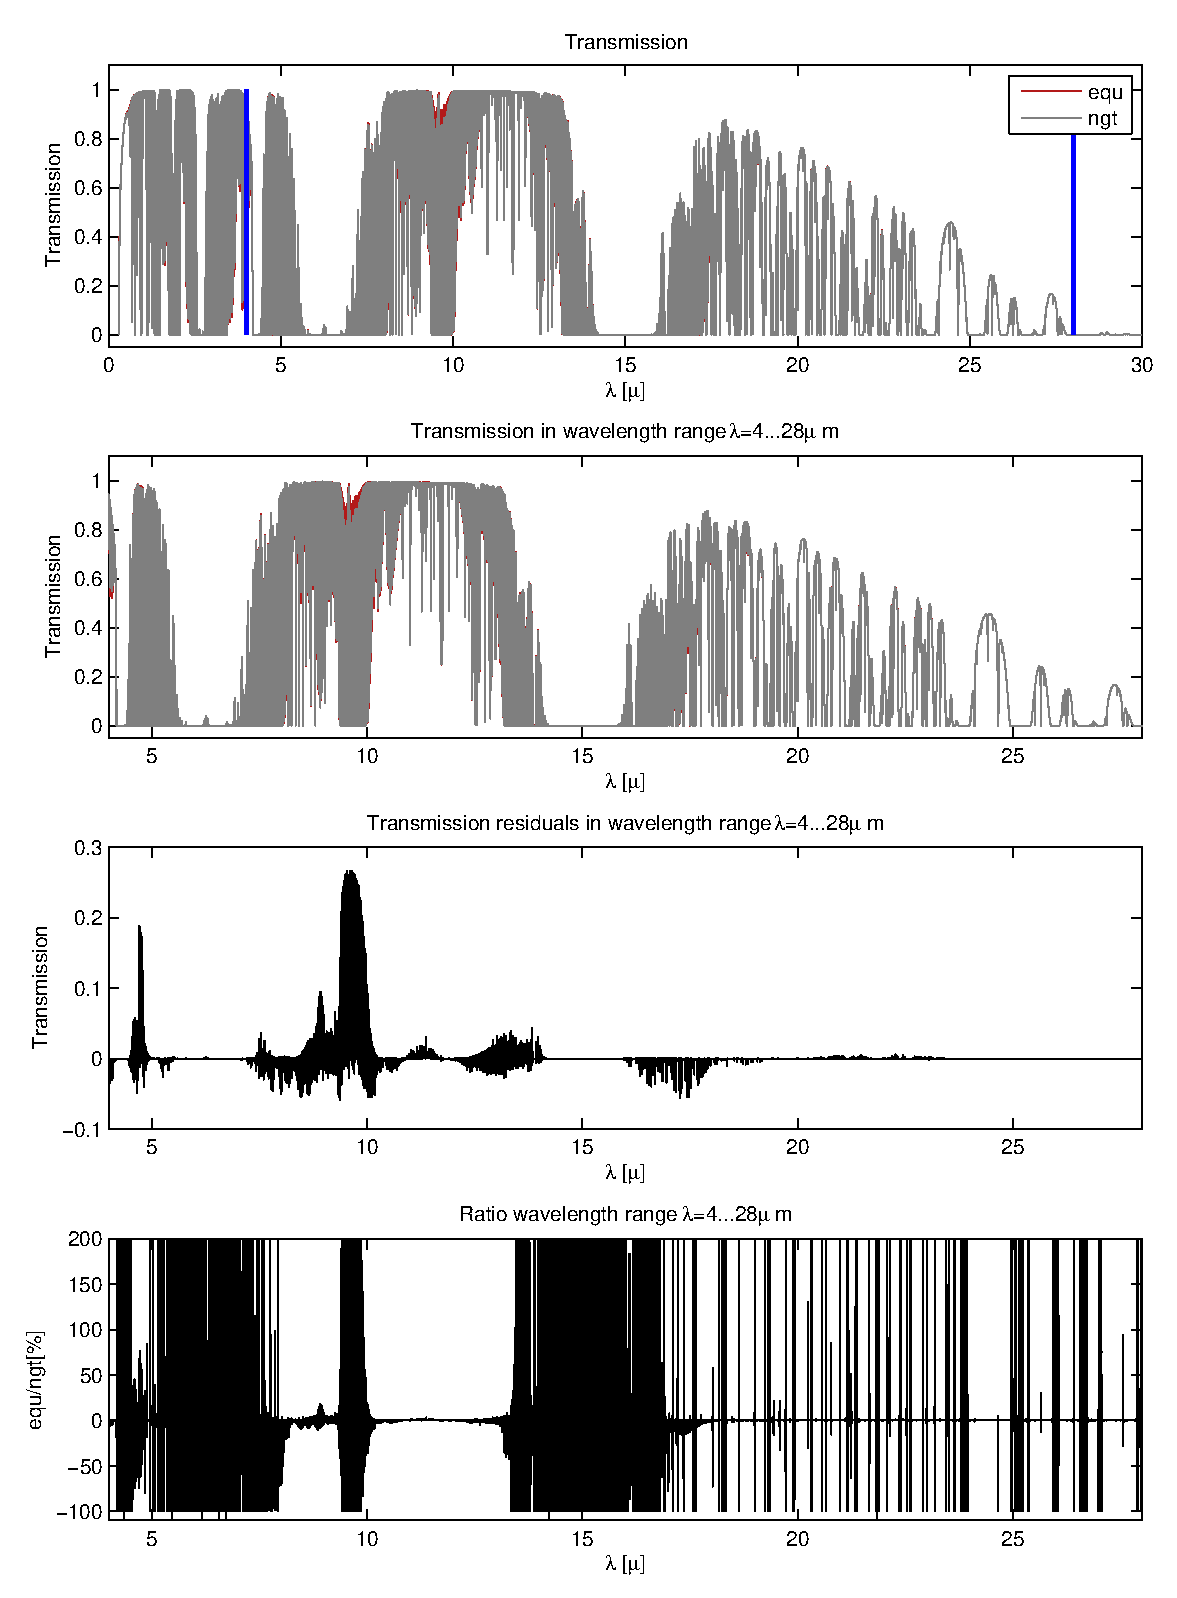
\psfig{file=figures/equ_ngt_4-28mu_tra.eps,width=0.75\textwidth}
    \caption{Same as Figure~\ref{fig:stdcomp_4-28_R}, but for the
    transmission.}
    \label{fig:stdcomp_4-28_T}
  \end{center}
\end{figure}
%-------------------------------------------------------------------------------

\clearpage

%-------------------------------------------------------------------------------
\subsubsection{GDAS profiles}\label{sec:gdas}
%-------------------------------------------------------------------------------
The \ac{GDAS} data provided by \ac{NOAA} are a model-based set of
meteorological data dedicated to weather forecast studies. The models are
archived by the \ac{ARL}, as a global, 1~degree latitude/longitude data set
based on pressure surfaces (starting from Dec.~2004). Apart from various
meteorological parameters for the surface, vertical profiles for 23 pressure
levels ranging from 0 to about 26\,km are provided for the geopotential height,
temperature, relative humidity, and wind components (not used in \mf) for three
dimensions. An example is shown in Figure~\ref{fig:gdas}.

%-------------------------------------------------------------------------------
\begin{figure}[ht]
  \begin{center}
    \begin{quote}
      \begin{small}
        \begin{verbatim}
# P[hPa] HGT[km] T[K]   RELHUM[%]
    903   0.971  294.5   49.9
    900   0.976  295.8   35.5
    850   1.467  293.7   30.9
    800   1.985  291.0   29.8
    750   2.533  288.2   27.4
    700   3.112  284.5   26.0
    650   3.726  280.7   18.8
    600   4.379  276.2   11.4
    550   5.077  271.4    8.7
    500   5.827  266.0    7.5
    450   6.638  259.9    7.5
    400   7.522  252.7   10.5
    350   8.494  244.7   25.1
    300   9.578  236.0   53.4
    250  10.813  227.0   66.5
    200  12.267  218.8   37.7
    150  14.069  209.2   17.3
    100  16.489  200.3   32.4
     50  20.571  206.1    0.0
     20  26.324  221.4    0.0
        \end{verbatim}
      \end{small}
    \end{quote}
    \caption{{\it GDAS profile} with columns for pressure, geoelevation,
    temperature, and relative humidity.}
    \label{fig:gdas}
  \end{center}
\end{figure}
%-------------------------------------------------------------------------------

The \mf\ software package provides the entire \ac{GDAS} data for the location
of Cerro Paranal from Dec.~2004 to Sep.~2013 on a 3\,h basis taken from the
\ac{NOAA}
archive\footnote{ \tt ftp://arlftp.arlhq.noaa.gov/pub/archives/gdas1/}.
Later dates (on a 6\,h basis) or data for a different site are automatically
downloaded from an online
archive\footnote{\tt http://nomad1.ncep.noaa.gov/pub/gdas/rotating/}.

%\clearpage

%-------------------------------------------------------------------------------
\subsubsection{ESO Meteo Monitor}\label{sec:emm}
%-------------------------------------------------------------------------------
The \ac{EMM} provides information on the local meteorological conditions at the
ESO sites La~Silla and Paranal. The data at Paranal are taken by a local meteo
station mounted on a 30\,m high mast installed in October 1984
\cite{meteomonitor}. This meteo station provides the following meteorological
information on a 20\,min average basis:

\begin{verbatim}
s1,d1 = wind speed (m/s) and direction (0=North, 90=East..)
        at 10m above ground (30m from 1998 onwards)
   rh = relative humidity (%) at 2m above ground
   t1 = air temperature (Celsius) at 2m above ground
   p  = pressure (mb) at 2m above ground
   td = dew point temperature (C) computed from rh and t1
\end{verbatim}

Starting from January 1st 1985, currently $\sim 400\,000$ data points are
measured with the following accuracy \cite{meteomonitor}:

\begin{verbatim}
wind direction: ~5.63deg
wind speed:     ~2% over 10m/s
temperature:    ~0.1deg
humidity:       linearity about 1%
seeing:         better than 10% above 0.25 arcsec
\end{verbatim}

The data can be retrieved online\footnote{\tt
http://archive.eso.org/asm/ambient-server} on a daily basis, or as download
provided by M.~Sarazin\footnote{\tt
http://www.eso.org/gen-fac/pubs/astclim/paranal/database/} and are
cumulatively shown in Figure~\ref{fig:meteomonitor}. Thus, for any requested
average time interval, like \eg\ December and January, ample measurements are
available. In compiling these data, care has to be taken to remove bad
measurements before further processing.

%-------------------------------------------------------------------------------
\begin{figure}[ht]
  \begin{center}
    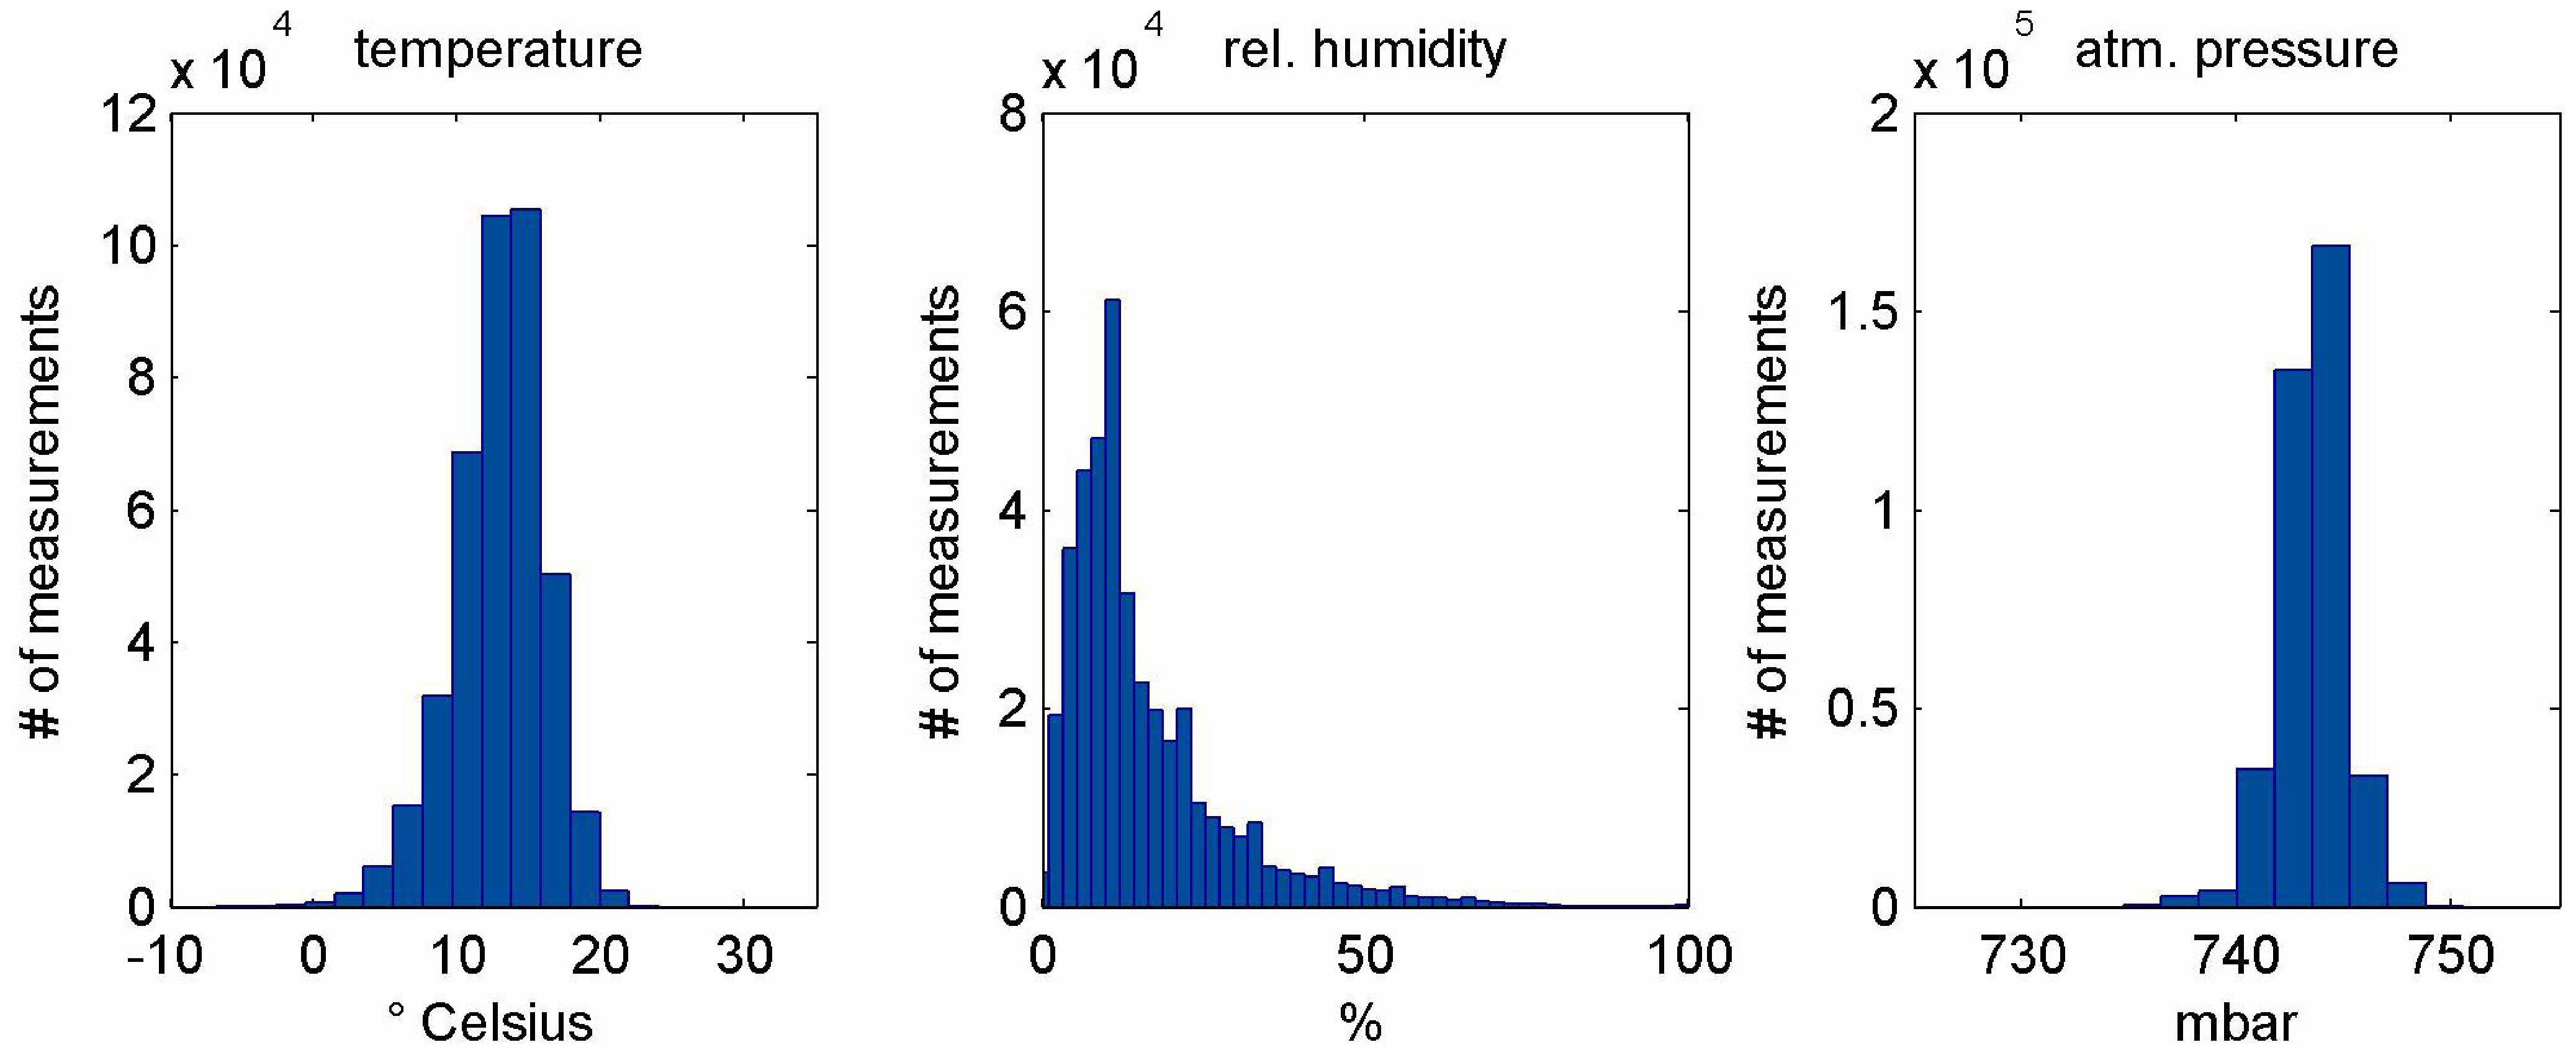
\psfig{file=figures/meteomonitor.eps,width=1.0\textwidth}
    \caption{Histograms of \ac{EMM} data (from Jan.~1985 to Jan.~2008).
{\it Left panel}: temperature; {\it middle panel}: relative humidity;
{\it right panel}: pressure.}
    \label{fig:meteomonitor}
  \end{center}
\end{figure}
%-------------------------------------------------------------------------------

\clearpage

%-------------------------------------------------------------------------------
\subsubsection{Processing of ESO Meteor Monitor data, GDAS, and MIPAS profiles}
\label{sec:processing}
%-------------------------------------------------------------------------------
The main disadvantage of the \ac{GDAS} profiles is that they do not represent
the local atmospheric conditions of the geographical position and height of the
observing site as accurately as provided by the \ac{EMM}, and even more so for
the MIPAS profiles. Therefore, one has to investigate how the three sources of
information can be merged into a single profile.

%-------------------------------------------------------------------------------
\paragraph*{GDAS profile processing}
\label{sec:gdas_processing}
%-------------------------------------------------------------------------------
The \ac{GDAS} profiles originate from a server at
\ac{NOAA}\footnote{http://140.90.198.158/pub/gdas/rotating/}. They are
retrieved via a dedicated software package \ac{GRIB} (see
Section~\ref{sec:installation}). \ac{GRIB} downloads a large data set
containing the specific \ac{GDAS} information for the requested point in time.
As this data set contains a model for the complete globe, subsequently, the
data points for the specified geolocation are extracted. Moreover, as the
\ac{GDAS} data are taken on a 3\,hr basis only, two profiles need to be
retrieved surrounding the requested point in time. The parameters
{\sc obsdate}, {\sc utc}, {\sc longitude}, and {\sc latitude} are required for
this task (see Section~\ref{sec:params}). They are usually provided by standard
and ESO FITS keywords. In the following, we will describe how the resulting two
profiles are combined to best match the date of the observations.

% As the download process from the web-server via \ac{GRIB} takes a considerable
% amount of time, \mf\ relies on two additional mechanisms to speed up the
% process. First of all, as the user works with his/her data set, the downloaded
% profiles are stored at a common location in the \mf\ directory tree
% (\verb|data/profiles/grib/| in {\sc basedir}, see Section~\ref{sec:params}).
% On subsequent calls of the routine, this location is first checked for the
% existence of the proper \ac{GDAS} profiles. 
If the profiles exist locally, no
download from the web-server is required. In addition, the \mf\ software
distribution contains a compilation of all Cerro Paranal \ac{GDAS} profiles for
the dates from Dec.~01, 2004 to Sep.~30, 2013. Thus, before requesting the data
from the web-server (in the case that they do not exist locally already), this
database is checked for the existence of the appropriate profiles. For
updates of this data set and the retrieval of data for other observing sites,
see Section~\ref{app:gdas}.

Unfortunately, the web-server does not provide \ac{GDAS} profiles for all
dates. Therefore, \mf\ incorporates a fall-back alternative to ensure
availability of \ac{GDAS} data in all occasions. To that end, the monthly
averaged profiles from the Cerro Paranal sky model are included as well (for a
detailed description see \cite{SM01UM} and Noll et al. \cite{NOL12}). If after
checking the local database or the web-server, a profile is still missing, the
best-matching profile for the two-month bins Dec.-Jan., Feb.-Mar., ...~are
taken. This is also done if the site is not Cerro Paranal.

The described procedure for the \ac{GDAS} profile retrieval is performed if
the parameter {\sc gdas\_prof} (see Section~\ref{sec:params}) is set to
``auto'', which is the default. As an alternative, a specific GDAS-like
profile (see Table~\ref{fig:gdas}) might be provided. Finally, it is possible
to avoid the use of GDAS profiles by setting {\sc gdas\_prof} to ``none''.

%-------------------------------------------------------------------------------
\paragraph*{Time averaged profiles}
\label{sec:time_average}
%-------------------------------------------------------------------------------
Typically, the requested observation date does not fall exactly onto a single
\ac{GDAS} time slot. Instead of simply retrieving the closest dataset the two
neighbouring profiles are obtained. In order to combine the two, a
time-weighted average is calculated, \ie\ performing a linear interpolation.

%-------------------------------------------------------------------------------
\paragraph*{Merging GDAS and MIPAS profiles}
\label{sec:gdas_mipas_merging}
%-------------------------------------------------------------------------------
Next, the resulting \ac{GDAS} profile is merged with the MIPAS standard
profile. To that end, the MIPAS profile is regridded to a new irregular height
grid with 50 levels (see Figure~\ref{fig:profile_levels}) spanning the whole
geoelevation range from 2-120\,km for Cerro Paranal. The \ac{GDAS} profile is
regridded to the same grid in the range 2-26\,km and then used to substitute
the respective columns in the MIPAS profile. In addition, the four height
levels from 20-26\,km are not only a simple substitute of the MIPAS data, but a
weighted mix of \ac{GDAS} and MIPAS profile, in order to provide a smooth
transition from one dataset to the other. The influence of the \ac{GDAS}
profile decreases with increasing height: 80\%, 60\%, 40\%, 20\% at 20\,km,
22\,km, 24\,km, 26\,km, respectively. Beyond 26\,km, no \ac{GDAS} information
is available.

The discussed fixed grid of layers is used if the parameter {\sc layers}
(see Section~\ref{sec:params}) is set to 1, which is the default. A value of
0 will cause the building of a natural grid consisting of all layers of the
MIPAS and the \ac{GDAS} profile. If local meteo data are used, the observer
altitude {\sc geoelev} is also added. The transition from \ac{GDAS} to MIPAS
is performed by means of a decrease of the relative difference of pressure,
temperature, and water vapour concentration of both profiles at the height of
the uppermost valid GDAS layer up to an altitude which is 1.2 times higher.
The resulting grid of layers is (slightly) more accurate than the fixed grid,
but also consists of a significantly higher number of levels.

%-------------------------------------------------------------------------------
\begin{figure}[ht]
  \begin{center}
    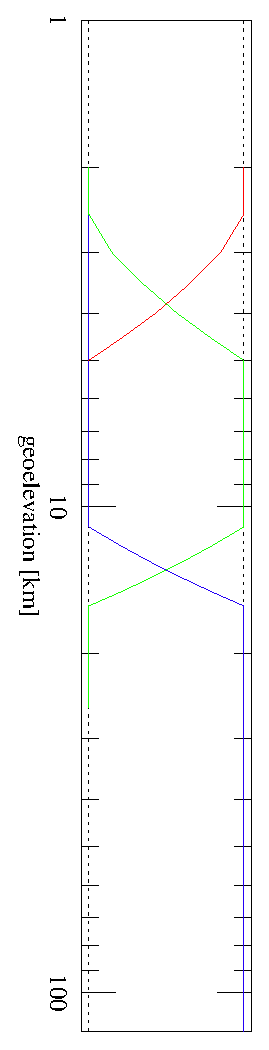
\psfig{file=figures/profiles.eps,height=1\textwidth,angle=90}
    \caption{{\it Composition of atmospheric profile:} relative importance of
    EMM data (red), \ac{GDAS} data (green) and MIPAS data (blue) as function of
    geoelevation. Note that the interface boundary of \ac{GDAS} and MIPAS data
    varies depending on the availability of the \ac{GDAS} data.}
    \label{fig:profile_levels}
  \end{center}
\end{figure}
%-------------------------------------------------------------------------------

%-------------------------------------------------------------------------------
\paragraph*{Combining GDAS/MIPAS profiles with EMM data}
\label{sec:emm_data}
%-------------------------------------------------------------------------------
Observed data from ESO telescopes provide on-site measurements at the ground
layer for pressure, temperature, and humidity originating from the ESO meteo
monitor at Cerro Paranal. A detailed study of the \ac{GDAS} data (see
Figure~\ref{fig:gdas_wind}), which represent the local troposphere, including
information concerning the dominant wind direction as a function of altitude
reveals a gradual reversal (rotation of 180$^\circ$) at a geoelevation of
5\,km, the so-called mixing altitude $h_{\mathrm{mix}}$ (see \cite{SM01UM}).
Beyond this altitude, the wind direction remains constant independent of the
observation date. Thus, it can safely be assumed that at this altitude the
influence of the local environment (as determined from the \ac{EMM} data) has
diminished.

In order to smoothly integrate the \ac{EMM} data, all \ac{GDAS} values for
pressure, temperature, and humidity below the altitude of the observatory are
set to the \ac{EMM} value. Values above the aforementioned mixing altitude are
left untouched. Intermediate values are linearly interpolated resulting in a
smooth transition. To this end, first, a logarithmically interpolated value of
the \ac{GDAS} data corresponding to the observatory's altitude $h_{\mathrm{tel}}$
is calculated for pressure, temperature, and humidity. These values describe
the reference point for the linear decrease of the relative difference between
\ac{EMM} and \ac{GDAS} data and in the interval $h_{\mathrm{tel}}-h_{\mathrm{mix}}$.

The resulting profile is a smooth combination of all input data, \ie\ MIPAS,
\ac{GDAS}, and \ac{EMM}.

The default mixing altitude of 5\,km can be manipulated by changing the
parameter {\sc emix} (see Section~\ref{sec:params}). This could be interesting
for other observing sites. Setting {\sc emix} to a value lower than the
observer altitude {\sc geoelev} causes a profile building without local meteo
data. In this case, the parameters {\sc pres}, {\sc temp}, and {\sc rhum} are
ignored.

%-------------------------------------------------------------------------------
\begin{figure}[ht]
  \begin{center}
    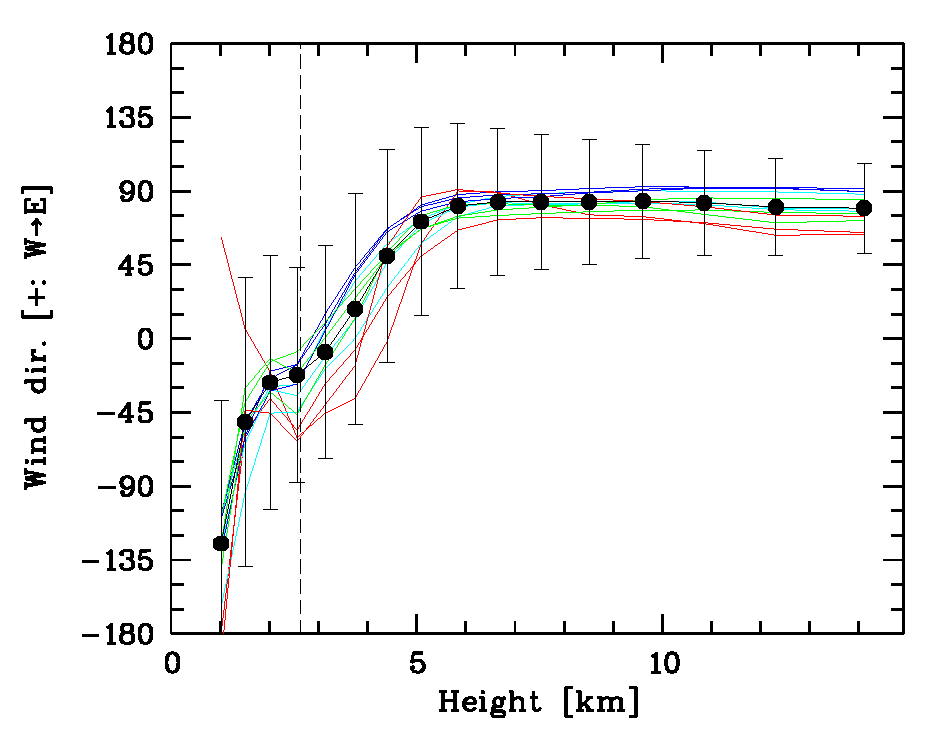
\psfig{file=figures/gdas_wdir_height_v.eps,width=0.7\textwidth}
    \caption{{\it \ac{GDAS} wind direction as function of geoelevation:} red,
cyan, blue, and green curves represent summer, autumn, winter, and spring,
respectively. The black symbols show the all year average with the
corresponding scatter. The vertical dashed line marks the geoelevation of
Paranal. At $\sim 5\,$km height, a constant plateau is reached.}
    \label{fig:gdas_wind}
  \end{center}
\end{figure}
%-------------------------------------------------------------------------------

%-------------------------------------------------------------------------------
\paragraph*{Scaling of the merged water vapour profile to a given PWV}
\label{sec:pwv_scaling}
%-------------------------------------------------------------------------------
The height profiles of the molecular abundances are defined by the atmospheric
standard profile. The only exception is water vapour, where the profile is a
combination of modelled and observed data as described above. The \ac{GDAS} and
\ac{EMM} data used cannot be controlled by the user. There might be cases where
this is not satisfying. For example, the user might be interested to use water
vapour columns derived from independent measurements for a better start
profile. For this purpose, \mf{} allows the user to enter a \ac{PWV} value
(parameter {\sc pwv}, see Section~\ref{sec:params}), which is used to scale the
merged water vapour profile. In this way, the input water vapour content of the
atmosphere can be fixed. Only the shape of the profile is then ruled by the
\ac{GDAS} and \ac{EMM} data. The profile scaling factor {\sc relcol}, which
is used in the context of the fitting procedure, refers to the modified
profile. By default, the {\sc pwv} option is switched off as indicated by a
value of -1.

%\clearpage

%-------------------------------------------------------------------------------
\subsection{Radiative transfer code}\label{sec:radcodes}
%-------------------------------------------------------------------------------
\mf\ uses the radiative transfer code Line-By-Line Radiative Transfer Model
(\lnflv{} / \lblrtmv), which is widely used in atmospheric and
climate research studies.

%-------------------------------------------------------------------------------
\subsubsection{Line File / Line-By-Line Radiative Transfer Model (LNFL/LBLRTM)}
\label{sec:lblrtm}
%-------------------------------------------------------------------------------
\ac{LBLRTM} is developed within the Radiative Transfer Working Group of the
\ac{AER} (see also Clough et al. \cite{CLO05}, \cite{AER}, and \cite{LBLRTM}).
It is publicly available. \ac{LBLRTM} can handle all molecules incorporated in
the {\tt aer\_v\_<version>} line parameter database \cite{LBLRTM} and offers a
wide range of possibilities to adjust input parameters (see
\cite{LBLRTM_instructions} for more details).

The \ac{AER} code package used here consists of two programmes: (a) the
"Line File" code \ac{LNFL}, which extracts user selected spectral lines from
the line parameter database, and provides these in appropriate form as input
for (b) the radiative transfer code \ac{LBLRTM}. Within \mf, the most recent
versions \lnflv{} and \lblrtmv{} are used.

Some \ac{LBLRTM} key features are (taken from \cite{LBLRTM}):

\begin{itemize}
  \item the Voigt line shape is used at all atmospheric levels with an
    algorithm based on a linear combination of approximating functions;
  \item it has been and continues to be extensively validated against
    atmospheric radiance spectra from the ultra-violet to the
    sub-millimeter;
  \item it incorporates the self- and foreign-broadened water vapour continuum
    model, MT\_CKD as well as continua for carbon dioxide, and for the
    collision induced bands of oxygen at 1600\,cm$^{-1}$ ($\lambda=6.25$\,\mum)
    and nitrogen at 2350\,cm$^{-1}$ ($\lambda=4.255$\,\mum);
  \item all parameters of the line database are used including the
    pressure shift coefficient, the halfwidth temperature dependence, and the
    coefficient for the self-broadening of water vapour;
  \item a version of the Total Internal Partition Function (TIPS) programme is
    used for the temperature dependence of the line intensities;
  \item the effects of CO$_2$ line coupling are treated as first order with
    the coefficients for carbon dioxide generated from Niro et al.
    \cite{NIR05};
  \item temperature dependent cross section data such as those available with
    the {\tt aer\_v\_<version>} database may be used to treat the absorption
    due to heavy molecules, \eg\ the halocarbons;
  \item an algorithm is implemented for the treatment of the variation of the
    Planck function within a vertically inhomogeneous layer as discussed in
    Clough et al. \cite{CLO92};
  \item algorithmic accuracy of \ac{LBLRTM} is approximately 0.5\% and the
    errors associated with the computational procedures are of the order of
    five times less than those associated with the line parameters so that the
    limiting error is that attributable to the line parameters and the line
    shape;
  \item its computational efficiency mitigates the computational burden of the
    line-by-line flux and cooling rate calculation (Clough et al.
    \cite{CLO92}), for example linear algebraic operations are used
    extensively in the computationally intensive parts of \ac{LBLRTM} so that
    vectorisation is particularly effective with a typical vectorised
    acceleration of 20;
  \item FFT instrument function with a choice of 9 apodisation functions;
  \item includes a realistic spectral sea surface emissivity model in the
    infrared (Masuda et al. \cite{MAS88}; Wu\&Smith \cite{WUS97});
  \item input atmospheric profiles in either altitude or pressure coordinates;
  \item interfaces with other radiative transfer models (like RRTM), and also
    the forward model for inversion algorithms (\eg\ Tropospheric Emission
    Spectrometer (TES) and Infrared Atmospheric Sounding Interferometer
    (IASI));
  \item these attributes provide spectral radiance calculations with
    accuracies consistent with the measurements against which they are
    validated and with computational times that greatly facilitate the
    application of the line-by-line approach to current radiative transfer
    applications.
\end{itemize}

In principle, the user can change the setup of the \ac{LBLRTM}. A reduced but
well documented list of input parameters and their default values is given by
the file ``config/lblrtm\_setup''. Some parameters are not fixed. They are
updated by other input data. For example, the wavelength range is given by
the input spectrum and possible cuts provided by the driver file (see
Section~\ref{sec:params}). A change of the fixed \ac{LBLRTM} input parameters
is only recommendable for those users, which have a very good knowledge of the
physics of atmospheric radiative transfer and/or \ac{LBLRTM}.

%-------------------------------------------------------------------------------
\subsubsection{{\tt aer} line database}\label{sec:molecs}
%-------------------------------------------------------------------------------
For calculating molecular spectra, the {\tt aer\_v\_<version>} database
\cite{LBLRTM} is used. It is built from \ac{HITRAN}~2008 \cite{HITRAN} and
contains several updates. Currently, it covers the full spectral range from
$0 - 25,232$\,cm$^{-1}$ (\ie\ up to $0.4\,\mu$m) provides spectral information
for 42 molecules. In total, more than 2,700,000 spectral lines are included.
The majority is based on modelled data. However, only those 30 molecules are
taken into account, which are present in the atmospheric standard profile. The
remaining ones are minor trace gases and do not contribute significantly
neither to radiance, nor transmission spectra (see Section~\ref{sec:spectra}).
Table~\ref{sec:molecs} provides an overview of all molecules based on the
{\tt aer} database (and known by \ac{LBLRTM}) and those contained in the
standard atmospheres (Column~4).

\begin{table*}[!ht]
\begin{center}
\caption{List of molecules as provided by the {\tt aer} line parameter database}
\label{tab:molecs}
\vspace{6pt}
\centering
\begin{tabular}{r | c | c | c | c}     % 5 columns
\hline\hline
\# of molecule & molecule & alt. name & std. atmosphere & \ac{LBLRTM} \\
\hline
1 & H$_2$O & Water & X & X \\
2 & CO$_2$ & Carbon dioxide & X & X \\
3 & O$_3$  & Ozone & X & X \\
4 & N$_2$O & Nitrous oxide & X & X \\
5 & CO  & Carbon monoxide & X & X \\
\hline
6 & CH$_4$ & Methane & X & X \\
7 & O$_2$  & Oxygen & X & X \\
8 & NO  & Nitric oxide & X & X \\
9 & SO$_2$ & Sulfur dioxide & X & X \\
10 & NO$_2$ & Nitrogen dioxide & X & X \\
\hline
11 & NH$_3$  & Ammonia & X & X \\
12 & HNO$_3$ & Nitric acid & X & X \\
13 & OH   & Hydroxyl &  & X \\
14 & HF   & Hydrogen fluoride &  & X \\
15 & HCl  & Hydrogen chloride &  & X \\
\hline
16 & HBr  & Hydrobromic acid &  & X \\
17 & HI   & Hydrogen iodide &  & X \\
18 & ClO  & Chlorine monoxide & X & X \\
19 & OCS  & Carbonyl sulfide & X & X \\
20 & H$_2$CO & Formaldehyde &  & X \\
\hline
21 & HOCl & Hypochlorous acid & X & X \\
22 & N$_2$   & Nitrogen & X & X \\
23 & HCN  & Hydrogen cyanide & X & X \\
24 & CH$_3$Cl & Chloromethane &  & X \\
25 & H$_2$O$_2$ & Hydrogen peroxide & X & X \\
\hline
26 & C$_2$H$_2$ & Acetylene & X & X \\
27 & C$_2$H$_6$ & Ethane & X & X \\
28 & PH$_3$  & Phosphine &  & X \\
29 & COF$_2$ & Carbonyl fluoride & X & X \\
30 & SF$_6$q  & Sulfur hexafluoride & X & X \\
\hline
31 & H$_2$S & Hydrogen sulfide  &  & X \\
32 & HCOOH & Formic acid &  & X \\
33 & HO$_2$ & Hydroperoxyl  &  & X \\
34 & O    & Oxygen &  & X \\
35 & ClONO$_2$q  &  & X & X \\
\hline
36 & NO+  & Nitrosonium &  & X \\
37 & HOBr &  &  & X \\
38 & C$_2$H$_4$ & Ethylene &  & X \\
39 & CH$_3$OH & Methanol &  & X \\
40 & BrO  &  &  & X \\
\hline
41 & C$_3$H$_8$ & Propane &  & X \\
42 & C$_2$N$_2$ & Cyanogen &  & X \\
\hline
\end{tabular}
\end{center}
\end{table*}

\clearpage

%-------------------------------------------------------------------------------
\subsection{Molecular spectra}\label{sec:spectra}
%-------------------------------------------------------------------------------
The process of fitting molecular spectra is a complex task, which requires
optimised input parameters. One of the key inputs for the fitting is the number
of molecules that are included in the fitting. Fewer molecules in the fitting
process result in the code finding a solution in significantly shorter amounts
of time. Also the fitting process is a lot more robust. However, if too few
molecules are included in the fit, the results may not provide a satisfying
residual for model and observation. Optimally, one should include exactly those
molecules in the fit, which will significantly contribute over the wavelength
range of interest.

To the end of providing some insight into what molecules are required for the
fit at a specific wavelength interval, in the following, we provide guidelines
with a specific focus on the test data provided with this software package for
the instruments CRIRES, VISIR, and X-Shooter (see Section~\ref{sec:pwv}).

We have computed spectra with \ac{LBLRTM} covering the complete wavelength
range from $0.3-30$\,\mum\ using all molecules (\ie\ C$_{2}$H$_{2}$,
C$_{2}$H$_{6}$, CH$_{4}$, CO$_{2}$, COF$_{2}$, CO, ClONO$_{2}$, ClO, F14,
H$_{2}$O$_{2}$, H$_{2}$O, HCN, HNO$_{3}$, HOCl, N$_{2}$O, N$_{2}$, NH$_{3}$,
NO$_{2}$, NO, O$_{2}$, O$_{3}$, OCS, SF$_{6}$, SO$_{2}$), individually, \ie\ one
at a time. At fixed wavelength, we have then calculated the normalised total
radiance/transmission (by summing up the contributions of all molecules and
subtracting the continuum) and the resulting relative importance of individual
molecules.

The Figures~\ref{fig:molecs_all}-\ref{fig:molecs_xshoo} shown in the Appendix,
give all molecules that, over the displayed wavelength range, exhibit at
fixed wavelength $\lambda$ a relative importance of at least 5\%. The molecular
data have been rebinned to 3000 data points for each individual wavelength
range. This results in a varying resolution and in more molecules becoming
important over smaller wavelength regimes. C$_{2}$H$_{6}$, \eg, has a few
significant lines in some of the wavelength ranges shown (\eg\
Figure~\ref{fig:molecs_crires}), but does not show up in the overview plot
(Figure~\ref{fig:molecs_all}). Typically, transmission (blue) and radiance
(red) plots do not differ significantly. Hence, we do not show them separately.
Note that these plots do not allow calculation of absolute fluxes.

These plots can be used to identify the important molecules over any wavelength
range. For the range shown in Figure~\ref{fig:molecs_crires}, \eg, the user
ought to include H$_{2}$O, CH$_{4}$, and O$_{3}$. The fitting might mildly profit
also from including C$_{2}$H$_{6}$.



%-------------------------------------------------------------------------------
\subsection{Thermal emission by telescope}\label{sec:greybody}
%-------------------------------------------------------------------------------
The telescope structure and the observing instrument cause unavoidable thermal
emission in the IR. In particular, the telescope main mirror is a significant
source of radiation. Hence, for radiance spectra, this background component has
to be considered. A simple approximation is the calculation of a grey body
spectrum, which equals a black body (BB) of temperature $T$ times a
wavelength-independent emissivity $\epsilon$. Since the emitting source, \ie\
the main mirror, also absorbs a fraction of $1 - \epsilon$ of the incoming
sky radiation, the relative contribution of the telescope emission to the
observed radiation is increased. Therefore, the apparent grey body radiation
in flux-calibrated spectra can be derived by
\begin{equation}
F_{\rm tel} = \frac{\epsilon}{(1 - \epsilon)} \,{\rm BB}(T).
\end{equation}
For $T$, \mf\ uses the temperature of the primary mirror (input parameter
{\sc m1temp}, see Section~\ref{sec:params}). Since the mirror temperature
is close to the ambient temperature of about 280-290\,K (Paranal), the grey
body emission is expected to be important at wavelengths longwards of the
$H$-band. The emissivity is a free fit parameter (see parameter {\sc telback}).
An initial value can be provided in the parameter file. The default value is
$0.1$.

%-------------------------------------------------------------------------------
\subsection{Adaptation of model to input spectrum}\label{sec:adaption}
%-------------------------------------------------------------------------------
A good correspondence of the calculated model spectrum and the observed
spectrum is usually prevented by the broadening of the spectral lines by the
instrument, small errors in the wavelength calibration, uncertainties in the
flux calibration in the case of emission spectra, or the non-flat standard star
continuum in the case of transmission spectra. Hence, these unavoidable
shortcomings of observed data have to be accounted for in the fitting
procedure. For this reason, \mf\ modifies the model spectrum using a
polynomial fit of the continuum and the wavelength grid. In addition, the model
gets convolved with a kernel mimicking the instrumental profile. In the
following, we discuss the fit parameters related to this adaptation process in
detail.

%-------------------------------------------------------------------------------
\subsubsection{The continuum}\label{sec:continuum}
%-------------------------------------------------------------------------------
The model spectrum is scaled by a polynomial of degree $n_\mathrm{c}$
({\sc cont\_n} in the parameter file; see Section~\ref{sec:params})
\begin{equation}
F_\mathrm{out}(\lambda) =
F_\mathrm{in}(\lambda) \, \sum_{i = 0}^{n_\mathrm{c}} a_i \lambda^i.
\end{equation}
For deriving the $n_\mathrm{c} + 1$ coefficients $a_i$, the zero point of the
wavelength grid is shifted to the centre of the fit range. For $a_0 = 1$ and
all other $a_i = 0$, the model spectrum remains unchanged. This is the default
configuration for the initial coefficients. In the parameter file, the
initial value of the constant term of the polynomial (parameter
{\sc cont\_const}) can be set manually. The continuum correction is carried
out independently for each fit range listed in the {\sc range\_include} file
if such a file is provided. A fit range (or the full spectrum) is further
split if it is distributed over more than one chip.

Before correcting the continuum, optionally a flux conversion is carried out.
Details on the options selected by the parameter {\sc flux\_unit} are given in
Section~\ref{sec:params}. If the required data units are not included in
{\sc flux\_unit}, this factor must be incorporated into the $a_0$ coefficient
of the polynomial. As a general rule, it is advisable to choose $a_0$ close to
the mean flux (emission) or maximum flux (transmission) of the input spectrum
(after consideration of {\sc flux\_unit}) to optimise the performance of \mf.

%-------------------------------------------------------------------------------
\subsubsection{The wavelength solution}\label{sec:wavegrid}
%-------------------------------------------------------------------------------
The wavelength grid of the model spectrum is adapted to that of the observed
spectrum by applying a Chebyshev polynomial of degree $n_\mathrm{w}$
({\sc wlc\_n} in the parameter file; see Section~\ref{sec:params})
\begin{equation}
\lambda' = \sum_{i = 0}^{n_\mathrm{w}} b_i t_i,
\end{equation}
where
\begin{equation}
t_i = \left\{ \begin{array}{ll}
1 & \textrm{for\ } i = 0 \\
\lambda & \textrm{for\ } i = 1 \\
2 \, \lambda \, t_{i-1} - t_{i-2} & \textrm{for\ } i \ge 2
\end{array} \right.
\end{equation}
and $\lambda$ ranging from -1 to 1. The temporary conversion of the wavelength
grid to a fixed interval results in coefficients $b_i$ independent of the
wavelength range and step size of the input spectrum. For $b_1 = 1$ and all
other $b_i = 0$, the model spectrum remains unchanged. This is the default
configuration for the initial coefficients. In the parameter file,
the initial value of the constant term of the polynomial (parameter
{\sc wlc\_const}) can be set manually. This parameter corresponds to a
wavelength shift relative to half the full wavelength range. For each chip or
FITS extension, the wavelength fit is carried out independently.

For checks or improvements of the input wavelength grid, the model wavelengths
rebinned to the input grid are provided in the results tables of \mf{} and
{\tt calctrans} (column ``mlambda'', see Section~\ref{sec:outputfiles}). The
wavelengths are always given in $\mu$m and vacuum. Note that the reliability of
this absolute wavelength calibration depends on the quality of the fit. Outside
the selected fitting ranges, the wavelengths have to be interpolated or
extrapolated by the Chebyshev polynomial. In particular, at optical and near-IR
wavelengths, where strong absorption bands suitable for fitting are rare, the
provided wavelengths have to be taken with care. For this reason, \mf{} does
not provide an automatic wavelength solution correction.

%-------------------------------------------------------------------------------
\subsubsection{The resolution}\label{sec:resolution}
%-------------------------------------------------------------------------------
The model spectrum is convolved with up to three different profiles in order to
get similar line shapes as in the observed spectrum. If a profile is not
desired, it can be skipped by setting its width and fit flag in the parameter
file to zero (see Section~\ref{sec:params}).

The first kernel is a simple boxcar
\begin{equation}
F_\mathrm{box}(\lambda) = \left\{ \begin{array}{ll}
1 & \textrm{for\ } -w_\mathrm{box}/2 \le \lambda \le w_\mathrm{box}/2 \\
0 & \textrm{for\ } \lambda < -w_\mathrm{box}/2 \cap \lambda > w_\mathrm{box}/2
\end{array} \right.
\end{equation}
which is adapted to the pixel scale and normalised to an integral of 1. In
the parameter file, the width $w_\mathrm{box}$ (parameter {\sc relres\_box}) has
to be given as fraction of the slit width, which is determined by the
parameters {\sc slitw}, the slit width in arcsec, and {\sc pixsc}, the pixel
scale in arcsec (see Section~\ref{sec:params}). By default, {\sc relres\_box}
is set to 1, \ie\ the slit width. The fit parameter {\sc relres\_box} can only
vary between 0 and 2.

The second convolution kernel is a Gaussian
\begin{equation}
F_\mathrm{gauss}(\lambda) = \frac{1}{\sigma \sqrt{2 \pi}}
\exp{\Bigg(-\frac{\lambda^2}{2 \sigma^2}\Bigg)}
\end{equation}
centred on 0, where
\begin{equation}
\sigma = \frac{w_\mathrm{gauss}}{2 \sqrt{2 \ln{2}}}.
\end{equation}
The FWHM $w_\mathrm{gauss}$ is given by the driver file parameter
{\sc res\_gauss} in pixels (see Section~\ref{sec:params}). It is restricted to
values below 100 pixels. The default value is 1 pixel. The number of pixels in
the kernel amounts to {\sc kernfac} (default: 3) times $w_\mathrm{gauss}$.

Finally, the third kernel is a Lorentzian
\begin{equation}
F_\mathrm{lorentz}(\lambda) = \frac{1}{\pi} \,
\frac{\lambda}{\lambda^2 + (w_\mathrm{lorentz}/2)^2}
\end{equation}
centred on 0, where $w_\mathrm{lorentz}$ is the FWHM. The width is adjusted by
the driver file parameter {\sc res\_lorentz}, which has to be provided in
pixels (see Section~\ref{sec:params}). It is restricted to values below 100
pixels. The default value is 1 pixel. The number of pixels in the kernel
amounts to {\sc kernfac} (default: 3) times $w_\mathrm{lorentz}$. Compared to a
Gaussian, the Lorentzian approaches the 0-level flux significantly slower, at
much larger distances from the maximum.

Note that width zero components can occur in typical conditions, \eg{} the line
profile is very close to a pure Lorentzian shape. If this is not intended, the
user should reduce the number of degrees of freedom by fixing individual fit
components. A zero here identifies a unity convolution (\ie{} no change
of the input spectrum).

The combination of a Gaussian and a Lorentzian is called a Voigt profile. The
flag {\sc kernmode} (see Section~\ref{sec:params}) allows the user to apply
only a single Voigt profile kernel, which is calculated by an approximate
formula that takes the FWHM of Gaussian and Lorentzian as input. In this case
({\sc kernmode} = 1), {\sc kernfac} gives the kernel size in FWHM of the
derived Voigt profile and not the FWHM of Gaussian and Lorentzian, as it is
done for the default mode of two independent convolutions ({\sc kernmode} = 0).
For the fit results, the {\sc kernmode} selection should be less important than
the relative contributions of boxcar, Gaussian, and Lorentzian to the fitted
line profile. Significant changes in the line profile can cause deviations in
the water vapour column of more than 10\% (cf. Section~\ref{sec:evaluation}).

The parameter {\sc varkern} allows the user to fit a kernel that linearly
increases with wavelength (see Section~\ref{sec:params}). If the flag is set to
1, this option is selected. It is suitable for dispersion-dominated kernels and
constant wavelength bins. In this case, the initial FWHM parameters are given
for the central wavelength of the full wavelength range (considering the data
of all chips). The default {\sc varkern}~=~0 assumes a constant kernel for the
entire wavelength range. This option is suitable for narrow wavelength ranges
and slit/object profile-dominated kernels.

Finally, the user can provide an optimised kernel by an ASCII file which is
provided by the parameter {\sc kernel\_file} (see Section~\ref{sec:params}).
If this option is used (\ie\ the default ``none'' is replaced by the
corresponding file name), the fixed input kernel overrules the creation of
a kernel based on boxcar, Gaussian, and Lorentzian components. Since there will
be no fit of the kernel shape and width, the line profile has to be known well.
Note that {\sc varkern}~=~1 will not have an effect, since the pixel-based
input kernel is wavelength independent.
